%
%   Data Clarification
%       - Plots...
%   
\clearpage
\section{Data clarification}
\label{section:data_clarify}








\subsection{Overview of features}

In this section, we provide a big picture of the our data via visualizations.

\subsubsection{Categorical features}

\begin{figure}[H]
    \centering
    \begin{subfigure}[b]{0.49\textwidth}
        \centering
        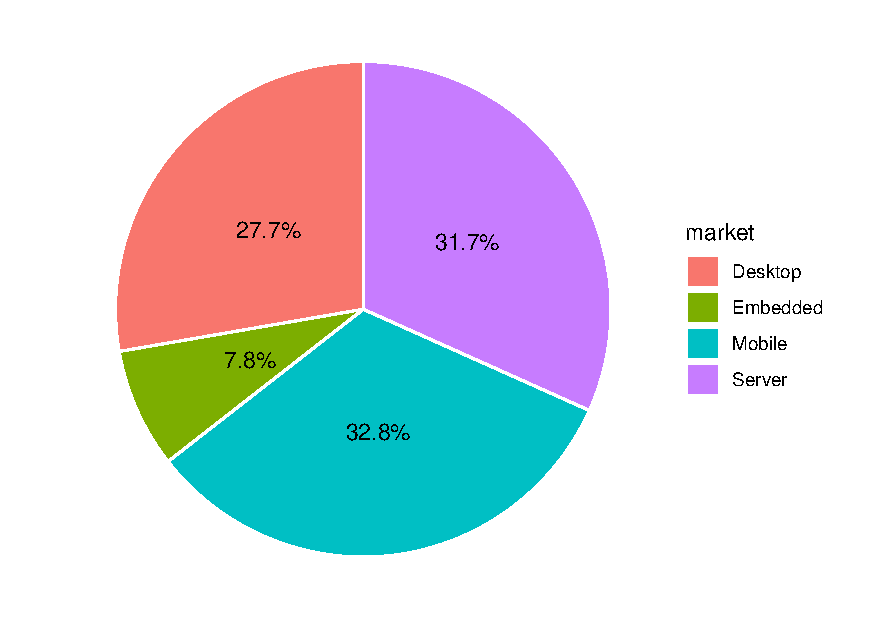
\includegraphics[width=\textwidth]{./graphics/pie_market.pdf}
        \caption{Pie of market share}
    \end{subfigure}
    \hfill
    \begin{subfigure}[b]{0.49\textwidth}
        \centering
        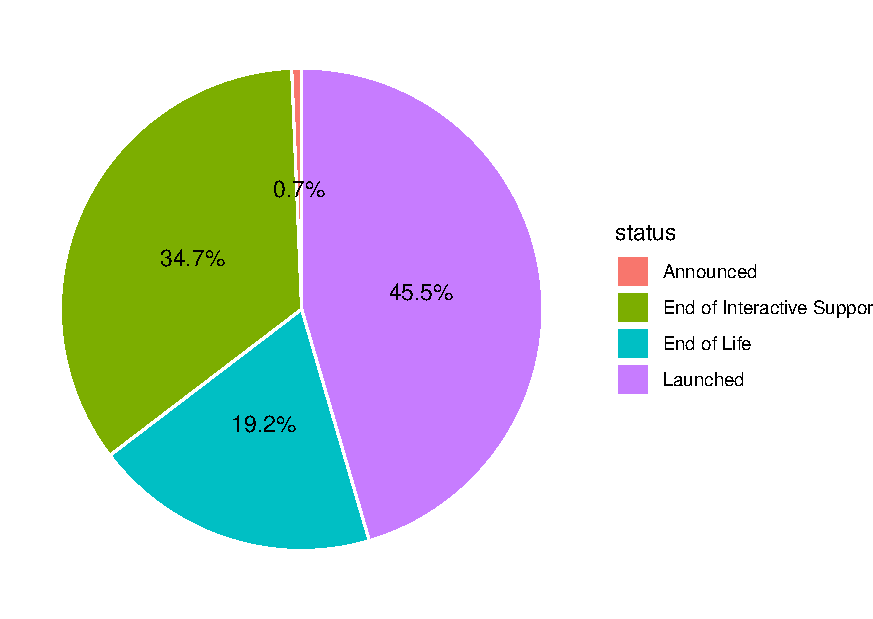
\includegraphics[width=\textwidth]{./graphics/pie_status.pdf}
        \caption{Pie of status}
    \end{subfigure}
    \caption{Pies of categorical features}
    \label{fig:pie_category}
\end{figure}

\textbf{[Figure \ref{fig:pie_category}]} Two obvious categorical features of our data are \textit{Market} and \textit{Status}.
\begin{itemize}
    \item In \textit{Market} feature, three primary shares of market are Desktop, Server and Mobile. Embedded constitues a very small
    proportion.
    \item In \textit{Status} feature, most of them are Launched, End of Life or End of interactive support. A tiny amound of Announce
    contribute modestly to total amount of CPU's model by provider Intel.
\end{itemize}

\subsubsection{Continuous features}

\begin{figure}[H]
    \centering
    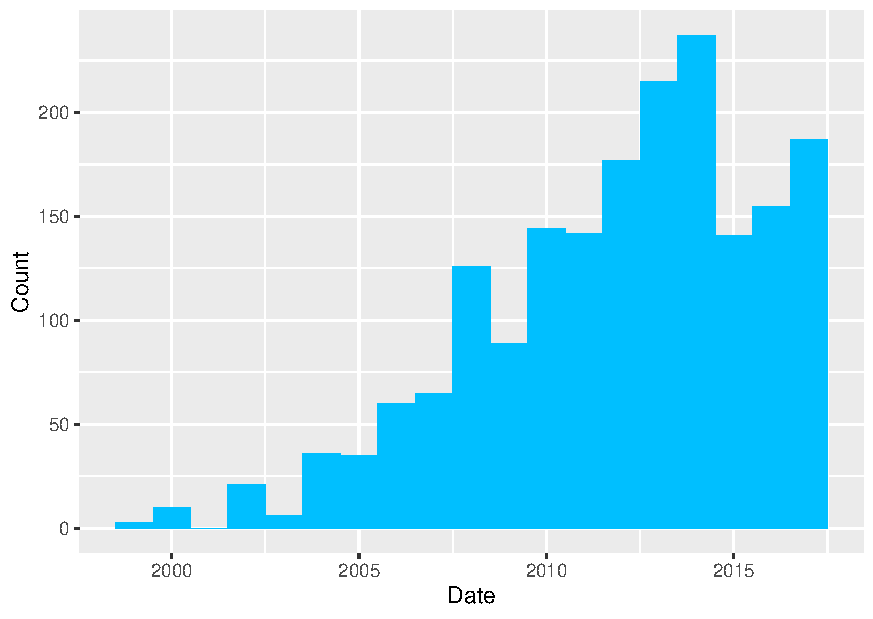
\includegraphics[width=0.5\textwidth]{./graphics/hist_ldate.pdf}
    \caption{Histogram of launch date}
    \label{fig:hist_ldate}
\end{figure}

\textbf{[Figure \ref{fig:hist_ldate}]} The \textit{Launch date} histogram shown that most of Intel's CPUs are launched recently, with two notable peaks at 2014 and 2017. The legacy
CPUs (before 2005) are only minor and can be treated as outliners if it is used in further analysis.

\begin{figure}[H]
    \centering
    \begin{subfigure}[b]{0.49\textwidth}
        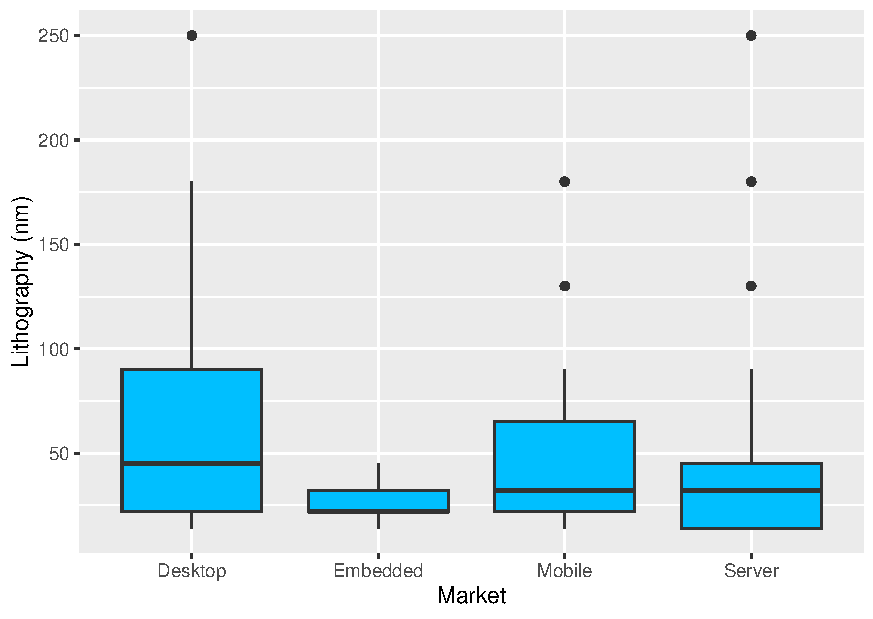
\includegraphics[width=\textwidth]{./graphics/box_litho.pdf}
        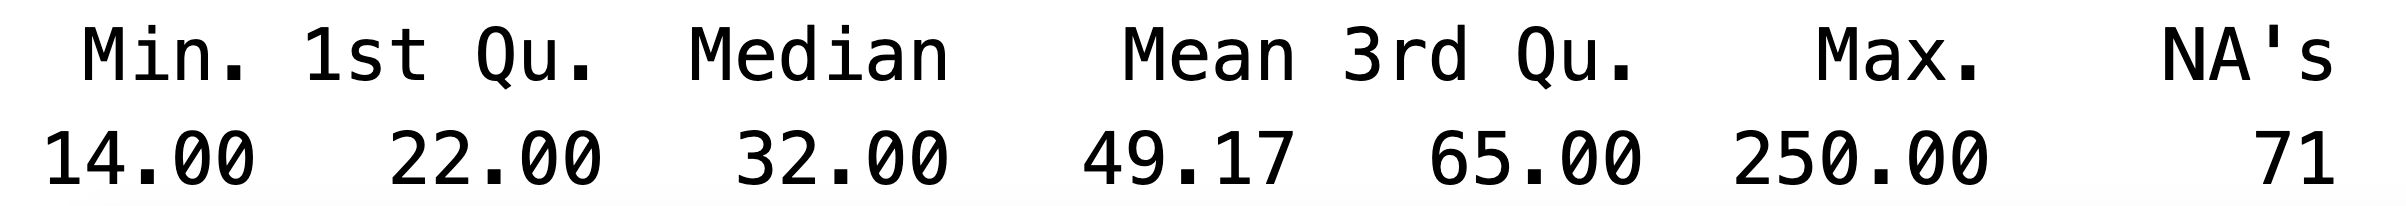
\includegraphics[width=\textwidth]{./graphics/sum_litho.png}
        \caption{Box plots and Summary of Lithography}
        \label{fig:box_litho}
    \end{subfigure}
    \hfill
    \begin{subfigure}[b]{0.49\textwidth}
        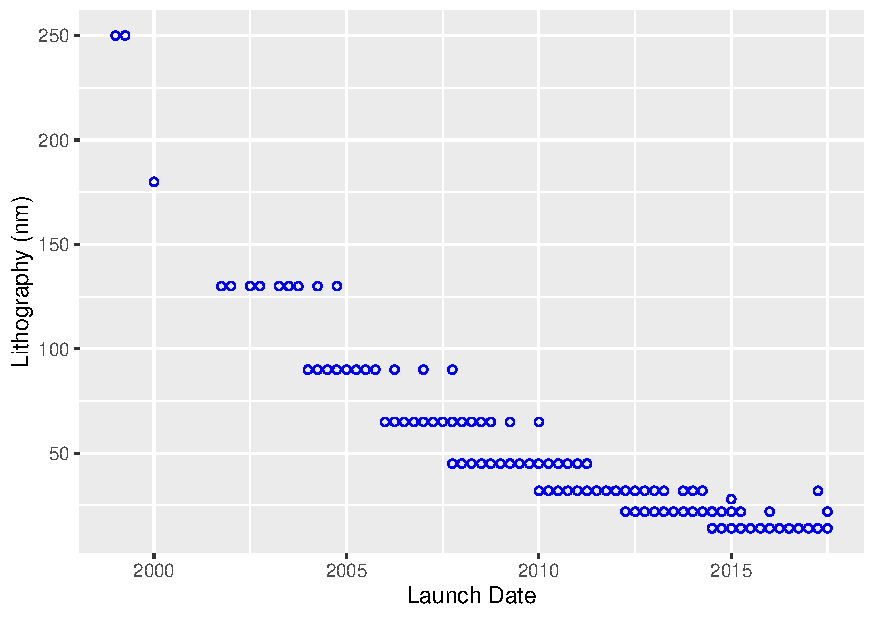
\includegraphics[width=\textwidth]{./graphics/scatter_litho.pdf}
        \caption{Plot of lithography over time.}
        \label{fig:scatter_litho}
    \end{subfigure}
    \caption{Lithography plots}
\end{figure}

\textbf{[Figure \ref{fig:box_litho}]} The box plot of \textit{Lithography} (chip printing technique) demonstrates interesting characteristics:
\begin{itemize}
    \item There was a large variance in the types of Lithography designed in Intel's Desktop processors, a smaller, but significant variance of 
    Mobile and Server are also observed. Embedded is less diverse, however, and also concentrates mostly on small \textit{Lithography} printings.

    \item The mean of \textit{Lithography}, in whatever market, is also approximately the same. That number might represents the most suitable 
    printing technique that is widely used among Intel's CPUs.
\end{itemize}

Overall, the most common \textit{Lithography} is $32 nm$. The best printing technique possible was $14 nm$ and the worst was $250 nm$. That large
number might come from old, legacy processors which were not designed with recent innovations in the Chip industry.

\textbf{[Figure \ref{fig:scatter_litho}]} The scatter plot of \textit{Lithography} with respect to \textit{Launch date} shown that the lithography
is getting smaller over time, and they are categorized into specific groups. So \textit{Lithography} can be treated as a Categorical feature as well
as Continuous feature.

\begin{figure}[H]
    \centering
    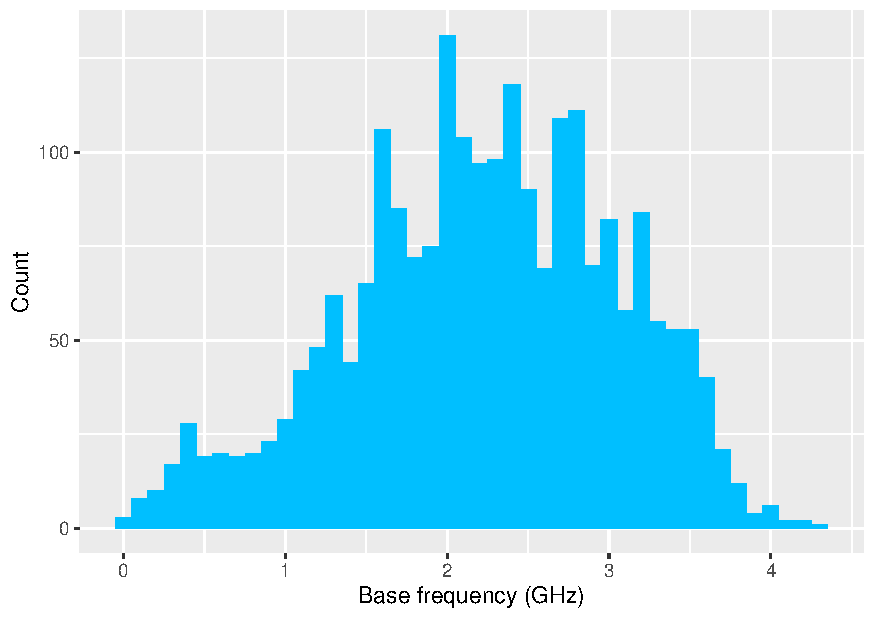
\includegraphics[width=0.5\textwidth]{./graphics/hist_bfreq.pdf}
    \caption{Histogram of Base Frequency}
    \label{fig:hist_bfreq}
\end{figure}

\textbf{[Figure \ref{fig:hist_bfreq}]} The most significant trend that could be observed in the \textit{Base frequency} histogram is its "normality".
In fact, this is expected because though higher frequency results in better performance, it has power and heat trade-offs. Thus, we see most choices of
frequencies concentrate around the mean of the distribution, which look pretty much like a bell-shape.

\begin{figure}[H]
    \centering
    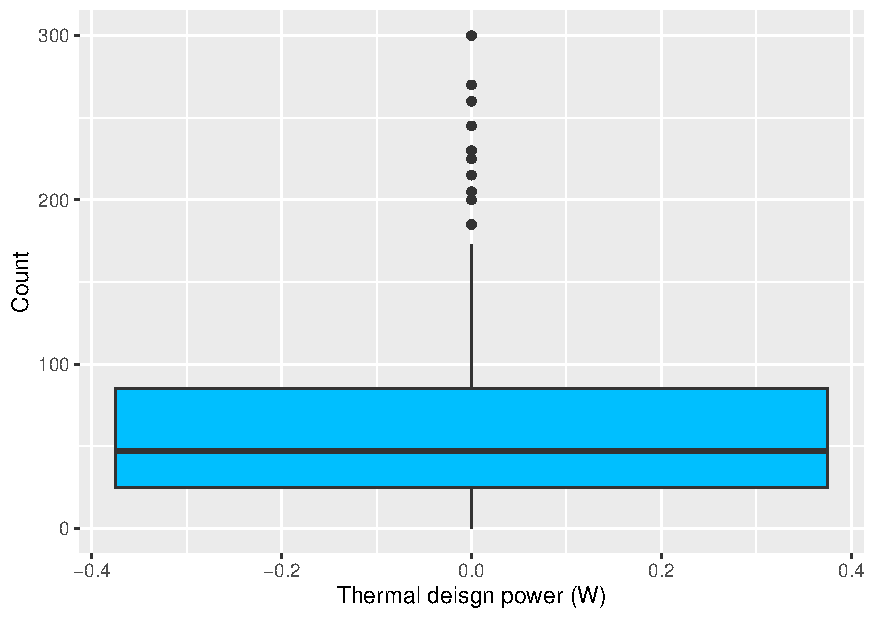
\includegraphics[width=0.5\textwidth]{./graphics/box_tdp.pdf}
    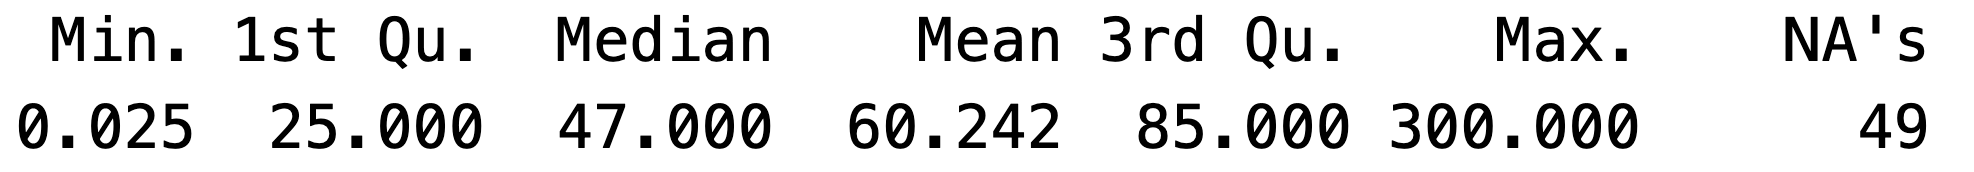
\includegraphics[width=0.5\textwidth]{./graphics/sum_tdp.png}
    \caption{Box plots and Summary of Thermal Design Power}
    \label{fig:box_tdp}
\end{figure}

\textbf{[Figure \ref{fig:box_tdp}]} The box plot of \textit{Thermal design power} is very market-dependent. While Embedded needed a very decent amount of
energy to release the heat, Server needed a lot, which is demonstrated by a much higher median. Server TDP's variance is also large, indicating
that there are many choices within this market. However, even so, its first quantile is still larger than most of the CPUs used in other markets.

% Should we plot memory bandwidth?
% \begin{figure}[H]
    %\centering
    %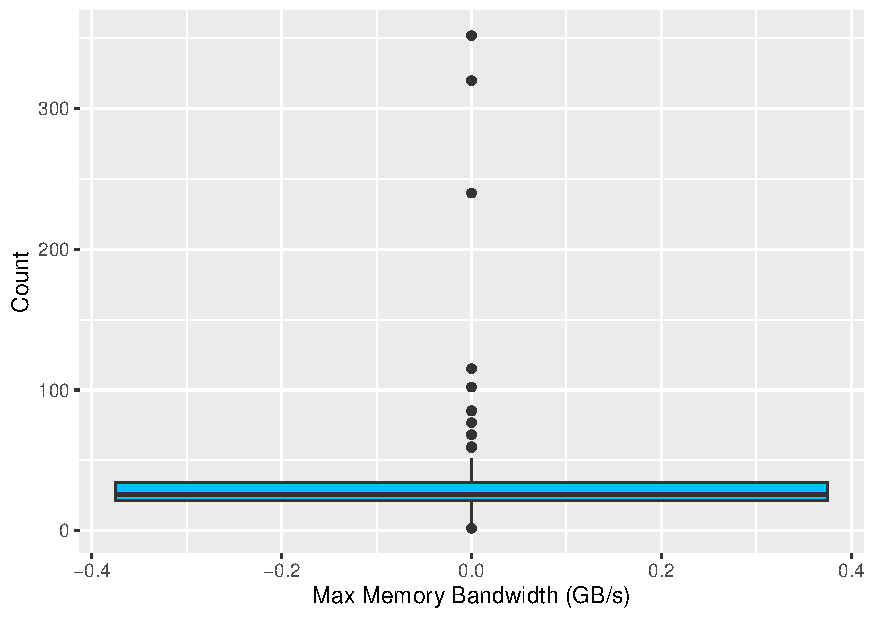
\includegraphics[width=0.5\textwidth]{./graphics/box_memband.pdf}
    %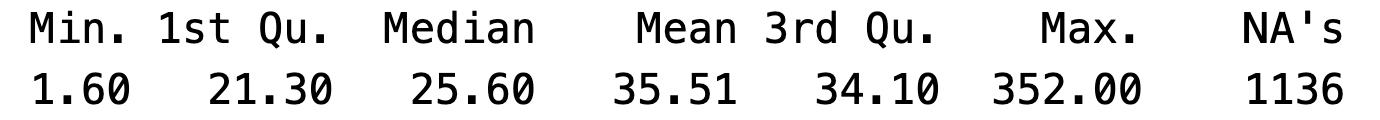
\includegraphics[width=0.5\textwidth]{./graphics/sum_memband.png}
    %\caption{Histogram of Maximum Memory Bandwidth}
%\end{figure}

% Should we plot Temperature? 
%\begin{figure}[H]
    %\centering
    %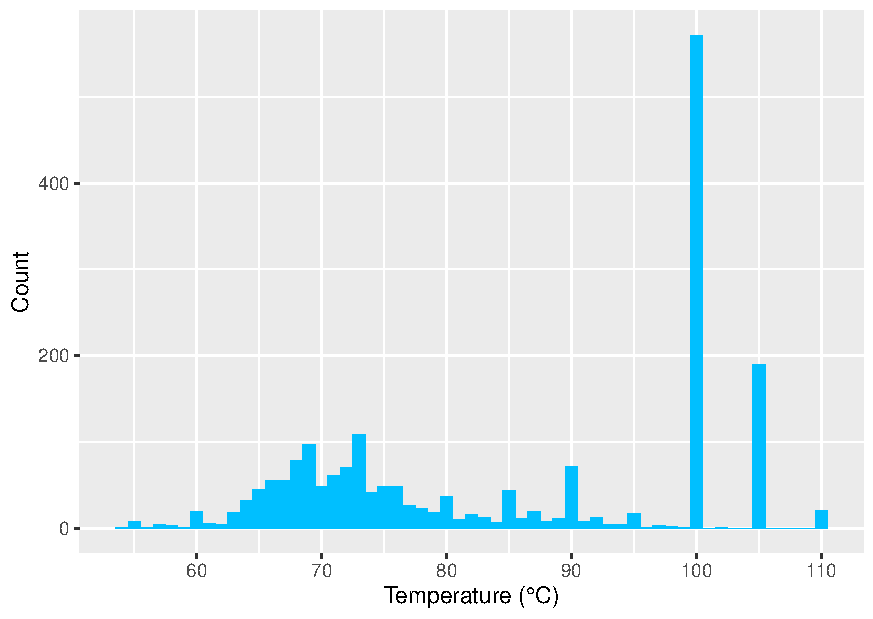
\includegraphics[width=0.5\textwidth]{./graphics/hist_temp.pdf}
    %\caption{Histogram of Temperature}
    %\label{fig:hist_temp}
%\end{figure}









\subsection{Analysis of features}

!!!! This is where the visualization for ANOVA and Regression kicks in. !!!!
